\section{Test Procedures}

\begin{figure}
	\centering
	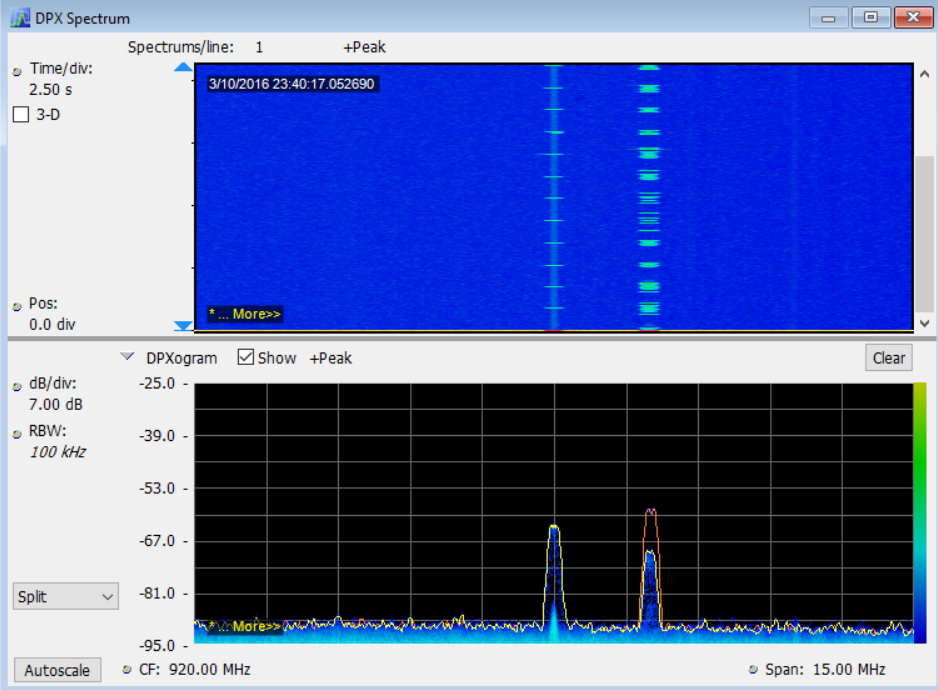
\includegraphics[scale=0.4]{FrequencyShift922-920}
	\caption{The result of using ALFRED to shift frequencies. One Node is left behind as the others move to the new channel.}
	\label{fig:freqshift}
\end{figure}


\begin{figure*}
	\centering
	\includegraphics[scale=0.5]{HopMessSmallest}
	\caption{The configuration used for the first set of tests.}
	\label{fig:HopMess}
\end{figure*}

\begin{figure*}
	\centering
	\includegraphics[scale=0.5]{NodeDrop}
	\caption{The configuration used for the second set of tests.}
	\label{fig:NodeDrop}
\end{figure*}

In order to characterize the platform we ran three sets of tests presented below. The first test characterizes data hopping from one node to the next. The second test demonstrates batman-adv's ability to switch routes based on the quality of each node. The final tests were used to examine A.L.F.R.E.D.'s ability to be used for exchanging frequency information from node to node. 

\subsection{Network Benchmarks}

The first test was used to investigate the overhead each node adds to the network. To examine how adding hops affects the network, we arranged the USRPs in a line so that each node only had one route to the following nodes.  We used a total of 5 nodes and this setup is shown in Figure \ref{fig:HopMess}. We staggered the transmit and receive frequencies of the nodes to ensure that nodes could only talk to their immediate neighbors, forcing the network into the proper configuration. The staggering of frequencies was needed to ensure each node would be unable to communicate to nodes other than its neighbors. 

 We then tested the setup at three different sets of frequencies, all within the Industrial, Scientific, and Medical (ISM) Band. We used different sets of ping tests in order to determine the number of dropped packets and the time it took to send the packets. We ran a standard ping test, one with reduced packet sizes, and one with increased time to live (TTL) setting. For a control group, two USRPs were connected together without batman-adv running. 


\subsection{Route Changes}

In a typical mesh environment, there will usually be more than one route from a source to a destination \cite{Akyildiz2009810}. In a traditional network, Batman-adv switches routes based on the quality of each available link. The test was designed to see if the same features would work in an SDRN. We initially setup four SDRs: a source, a destination, and two nodes to connect them. We give a significantly larger gain to the first node, in order to see if Batman-adv will recognize that this is a stronger path to the destination. Then, once the route is placed into the routing table, we lower the gain to 0 in order to force a transition to the other node. We then see if batman-adv is still able to find the new route even though it is running on a USRP. This setup is shown in Figure \ref{fig:NodeDrop}.



\subsection{Frequency Distribution}

In the final test, we tested to see if A.L.F.R.E.D. would properly relay frequency changes over the mesh to other nodes. The user would increase or decrease the frequency using the web interface in order to simulate a cognitive radio making a decision to change to a new frequency. If A.L.F.R.E.D. was able to exchange the information properly, then the routing table will still show all connected nodes. We also use a Tektronix RSA306 Spectrum Analyzer in order to see that the transmission is occurring on the new frequency. If A.L.F.R.E.D. was not able to relay the information to all nodes, then some change to the new frequency while others remain. This would be reflected in the output from the spectrum analyzer. 